% AI Tool Kart — News Agent: parameter quick-reference.
% Companion to AGENT_ARTICLE_JUDGEMENT_CRITERIA.tex (55pp). Values identical.

\documentclass[10pt,a4paper]{article}

\usepackage[T1]{fontenc}
\usepackage{lmodern}
\usepackage[margin=1.9cm,top=1.7cm,bottom=1.9cm]{geometry}
\usepackage{xcolor}
\usepackage{booktabs}
\usepackage{tabularx}
\usepackage{array}
\usepackage{amsmath}
\usepackage{enumitem}
\usepackage{ragged2e}
\usepackage{tikz}
\usetikzlibrary{arrows.meta,positioning,calc}
\usepackage[most]{tcolorbox}
\usepackage{titlesec}
\usepackage[hidelinks]{hyperref}

\definecolor{nv}{HTML}{1F2A44}
\definecolor{st}{HTML}{9B2C3A}
\definecolor{hd}{HTML}{8A6100}
\definecolor{go}{HTML}{1F6F4A}
\definecolor{ac}{HTML}{4C5FD5}
\definecolor{sf}{HTML}{EEF1FA}
\definecolor{gy}{HTML}{5A6272}

\titleformat{\section}{\normalfont\large\bfseries\color{nv}}{\thesection}{0.6em}{}
\titlespacing*{\section}{0pt}{1.05em}{0.35em}
\titleformat{\subsection}{\normalfont\normalsize\bfseries\color{gy}}{\thesubsection}{0.5em}{}
\titlespacing*{\subsection}{0pt}{0.7em}{0.25em}

\setlength{\parindent}{0pt}
\setlength{\parskip}{0.35em}
\renewcommand{\arraystretch}{1.14}
\tolerance=2500 \emergencystretch=3em \exhyphenpenalty=0 \hbadness=4000
\setlist[itemize]{leftmargin=1.1em,itemsep=0.1em,topsep=0.15em,parsep=0pt}

\newcommand{\vr}[1]{\texttt{\footnotesize\hyphenpenalty=0\exhyphenpenalty=0\relax #1}}
\newcommand{\cd}[1]{\texttt{\footnotesize\hyphenpenalty=0\exhyphenpenalty=0\relax #1}}
\newcommand{\us}{\_\discretionary{}{}{}}
\newcommand{\D}{\textcolor{go}{\textbf{D}}}
\newcommand{\Lm}{\textcolor{ac}{\textbf{L}}}
\newcommand{\LD}{\textcolor{hd}{\textbf{L$\rightarrow$D}}}
\newcommand{\BL}{\textcolor{st}{\textbf{block}}}
\newcommand{\AD}{\textcolor{hd}{advisory}}
\newcommand{\DF}{\textcolor{hd}{\textbf{defer}}}

\newtcolorbox{note}{enhanced,breakable,colback=sf,colframe=ac,boxrule=0pt,
  leftrule=2.5pt,arc=1pt,left=6pt,right=6pt,top=4pt,bottom=4pt}
\newtcolorbox{warn}{enhanced,breakable,colback=st!6,colframe=st,boxrule=0pt,
  leftrule=2.5pt,arc=1pt,left=6pt,right=6pt,top=4pt,bottom=4pt}

\begin{document}

\begin{center}
{\LARGE\bfseries\color{nv} AI Tool Kart — News Agent}\\[0.25em]
{\large\bfseries Parameter, Threshold and Gate Summary}\\[0.4em]
{\footnotesize\color{gy} Quick reference. Companion to \cd{AGENT\us ARTICLE\us JUDGEMENT\us CRITERIA.pdf} (55 pp).\\
All values read from the implementation; identical to the detailed document.}
\end{center}

\vspace{-0.3em}
\begin{center}\footnotesize
\fbox{\begin{minipage}{0.96\textwidth}\centering
\textbf{Decision-source key:}\quad
\D~= deterministic code \quad\textbullet\quad
\Lm~= decided by the LLM \quad\textbullet\quad
\LD~= LLM-generated, code-enforced\\[0.2em]
\textbf{Gate key:}\quad \BL~= prevents publication \quad\textbullet\quad
\DF~= pauses, story survives \quad\textbullet\quad \AD~= reported only
\end{minipage}}
\end{center}

{\footnotesize\setlength{\parskip}{0pt}
\renewcommand{\contentsname}{\normalsize\color{nv}Contents}
\tableofcontents}

\vspace{0.4em}

% =============================================================================
\section{Pipeline Overview}

\begin{center}\footnotesize
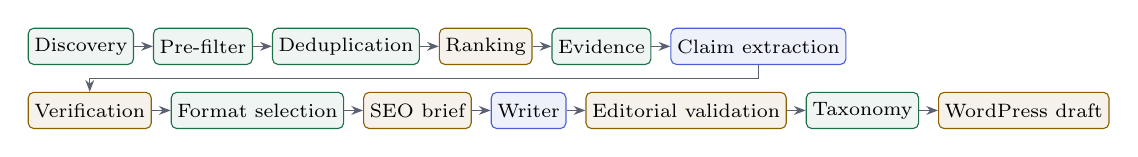
\begin{tikzpicture}[node distance=2.4mm,
  b/.style={draw=go,fill=go!7,rounded corners=2pt,inner sep=2.2pt,font=\scriptsize,minimum height=4.6mm},
  l/.style={draw=ac,fill=sf,rounded corners=2pt,inner sep=2.2pt,font=\scriptsize,minimum height=4.6mm},
  m/.style={draw=hd,fill=hd!8,rounded corners=2pt,inner sep=2.2pt,font=\scriptsize,minimum height=4.6mm},
  a/.style={-{Stealth[length=1.5mm]},draw=gy}]
\node[b](n1){Discovery};
\node[b,right=of n1](n2){Pre-filter};
\node[b,right=of n2](n3){Deduplication};
\node[m,right=of n3](n4){Ranking};
\node[b,right=of n4](n5){Evidence};
\node[l,right=of n5](n6){Claim extraction};
\node[m,below=3.4mm of n1.south west,anchor=north west](n7){Verification};
\node[b,right=of n7](n8){Format selection};
\node[m,right=of n8](n9){SEO brief};
\node[l,right=of n9](n10){Writer};
\node[m,right=of n10](n11){Editorial validation};
\node[b,right=of n11](n12){Taxonomy};
\node[m,right=of n12](n13){WordPress draft};
\foreach \i/\j in {n1/n2,n2/n3,n3/n4,n4/n5,n5/n6,n7/n8,n8/n9,n9/n10,n10/n11,n11/n12,n12/n13}
  \draw[a](\i)--(\j);
\draw[a](n6.south)--++(0,-1.7mm)-|($(n7.north)+(0,1.7mm)$)--(n7.north);
\end{tikzpicture}
\end{center}

\vspace{-0.5em}
\begin{center}\footnotesize
\begin{tabularx}{\textwidth}{@{}l l >{\RaggedRight}X@{}}
\toprule
\textbf{Stage} & \textbf{Type} & \textbf{Decision made} \\
\midrule
Discovery & \D & Which feeds are read; per-source item cap \\
Pre-filter & \D & Freshness, banned domain, title length, hard-rejected topic, topic prior \\
Deduplication & \D & Canonical-URL identity; title-similarity clustering \\
Ranking & mixed \LD & LLM scores relevance/importance; code computes trust + freshness, applies weights and floors \\
Evidence & \D & Which pages are fetched, in what order; sufficiency rule \\
Claim extraction & \Lm & Atomic claims + claim type (bounded by closed schema) \\
Verification & mixed \LD & LLM assigns support level; tier rules downgrade; code applies 4 story gates \\
Format selection & \D & brief / standard / analysis from verified-claim and publisher counts \\
SEO brief & mixed \LD & LLM proposes metadata; code re-derives slug, filters links, validates grounding \\
Writer & \Lm & Prose only, from verified claims; code renders HTML, slug, tags \\
Editorial validation & mixed \LD & LLM verdict; code overrides on deterministic issues and confidence floor \\
Taxonomy & \D & Category allowlist; tag validation, normalisation, cap \\
WordPress draft & \D & 9 final checks; \cd{status = draft} hardcoded \\
\bottomrule
\end{tabularx}
\end{center}

% =============================================================================
\section{Discovery / Source Parameters}

\begin{center}\footnotesize
\begin{tabularx}{\textwidth}{@{}>{\RaggedRight}p{3.5cm} >{\RaggedRight}X c c >{\RaggedRight}p{4.1cm}@{}}
\toprule
\textbf{Parameter} & \textbf{Current value / rule} & \textbf{Src} & \textbf{Blocking?} & \textbf{Failure behaviour} \\
\midrule
Source registry & 17 registered, \textbf{10 enabled} (7 Tier 1, 3 Tier 2); single file \cd{src/sources/registry.ts} & \D & --- & Adding a source is config, not code \\
\cd{enabled} & \cd{true|false} per source & \D & \BL & Source is not read at all \\
\cd{id} & Stable string, e.g. \cd{openai-news} & \D & --- & Used for tier/publisher lookup \\
\cd{trustTier} & \cd{1|2|3}; travels with every item into verification & \D & \BL & Drives evidence + claim rules \\
Trust score by tier & Tier 1 = 10, Tier 2 = 7, Tier 3 = 3 & \D & --- & Feeds the weighted score \\
\cd{type} & \cd{rss} \textbar{} \cd{api} \textbar{} \cd{web}; only \cd{rss} implemented \& enabled & \D & \BL & All \cd{web} entries disabled \\
\cd{maxItemsPerRun} & Per-source override; set to \textbf{15} for GitHub Changelog and AWS ML Blog & \D & \DF & Excess items not ingested this run \\
\vr{AGENT\us MAX\us ITEMS\us PER\us SOURCE\us PER\us RUN} & Default \textbf{25} (global fallback) & \D & \DF & Excess items not ingested this run \\
\cd{publishedAt} & From feed; used for freshness & \D & --- & See \S3 for missing/invalid dates \\
Source fetch failure & Isolated per source; counted in \cd{sourcesFailed} & \D & \textbf{no} & Run continues with other sources \\
Source parse failure & Same isolation; body never logged & \D & \textbf{no} & Run continues \\
Fetch order & Sequential, not parallel & \D & --- & --- \\
HTTP guard & HTTPS only, private/link-local addresses rejected, \textbf{3} redirects max, \vr{AGENT\us HTTP\us TIMEOUT\us MS} = 15000, \vr{AGENT\us MAX\us RESPONSE\us BYTES} = 2500000 & \D & \BL & URL rejected; \cd{URL\us REJECTED} \\
\bottomrule
\end{tabularx}
\end{center}

\textbf{Disabled sources (reason recorded, not guessed URLs):} Anthropic, Meta AI, Mistral, Microsoft, Runway (Tier 1 --- no stable feed / 404 / 410); Ars Technica (Tier 2 --- feed valid, section too broad). \textbf{No Tier 3 source is configured}; Tier 3 remains the default tier for any unrecognised host.

% =============================================================================
\section{Freshness / Initial Pre-filter}

All checks below run \textbf{before the first LLM call} and are fully \D.

\begin{center}\footnotesize
\begin{tabularx}{\textwidth}{@{}>{\RaggedRight}p{4.2cm} >{\RaggedRight}X c >{\RaggedRight}p{4.3cm}@{}}
\toprule
\textbf{Check / config name} & \textbf{Value / rule} & \textbf{Gate} & \textbf{Reason code on failure} \\
\midrule
\cd{maxStoryAgeHours} & \textbf{96 h}, measured from the \emph{freshest} backing item & \BL & \cd{stale (}\textit{n}\cd{h old)} \\
Missing / unparseable date & \cd{publishedAt} omitted; age falls back to \cd{discoveredAt} (treated as fresh) & --- & --- \\
Future-dated item & Rejected beyond \textbf{6 h} clock skew; date dropped, falls back to \cd{discoveredAt} & --- & --- \\
\cd{minTitleLength} & \textbf{12} characters; checked at ingestion and again at prefilter & \BL & \cd{title-too-short} \\
\cd{BANNED\us DOMAINS} & \textbf{9} hosts (\cd{news.google.com}, \cd{medium.com}, \cd{msn.com}, \cd{yahoo.com}, \cd{flipboard.com}, \cd{benzinga.com}, \cd{investing.com}, \cd{analyticsinsight.net}, \cd{marktechpost.com}) & \BL & \cd{banned-domain} \\
\cd{EXCLUDED\us TOPICS} (hard) & \textbf{5} rules: \cd{stock}, \cd{doom}, \cd{clickbait}, \cd{listicle}, \cd{horoscope-noise} & \BL & \cd{excluded-topic:}\textit{id} \\
\cd{EXCLUDED\us TOPICS} (soft) & \textbf{3} rules: \cd{rumor} $-3$, \cd{celebrity} $-3$, \cd{unrelated-funding} $-1.5$ & \AD & Score penalty only \\
\cd{INCLUDED\us TOPICS} & \textbf{10} rules, weights $+1$ to $+2.5$ (highest: \cd{mcp} $+2.5$) & \AD & Score bonus only \\
\cd{AUDIENCE\us ENTITIES} & 43-entry vocabulary; $+0.5$ per hit, \textbf{capped at 3 hits} ($+1.5$ max) & \AD & Score bonus only \\
Terminal story status & Not \cd{published}, not \cd{rejected}, no \cd{duplicateOfStoryId} & \BL & \cd{already-published}, \cd{previously-rejected}, \cd{duplicate-of-}\allowbreak\cd{existing-story} \\
Has backing items & $\geq 1$ news item & \BL & \cd{no-source-items} \\
\bottomrule
\end{tabularx}
\end{center}

% =============================================================================
\section{Deduplication}

\begin{center}\footnotesize
\begin{tabularx}{\textwidth}{@{}>{\RaggedRight}p{3.2cm} >{\RaggedRight}X c@{}}
\toprule
\textbf{Level / parameter} & \textbf{Rule as implemented} & \textbf{Src} \\
\midrule
Canonical URL & Forced \cd{https}; host lowercased with \cd{www.}/\cd{m.}/\cd{amp.} stripped; $\sim$40 tracking params removed (\cd{utm\us *}, \cd{fbclid}, \cd{gclid}, \cd{pk\us *}, \ldots); redirect wrappers unwrapped \textbf{one level}; AMP/\cd{index.html} suffixes stripped; remaining params sorted; fragment discarded & \D \\
L1/L2 uniqueness & Canonical URL is a \textbf{database uniqueness constraint} on \cd{news\us items} & \D \\
Title normalisation & Publisher masthead stripped; stop-words removed; 30+ announcement verbs folded to one token (\cd{launch}/\cd{update}) & \D \\
Title similarity & $\max(0.7 \cdot \text{token Jaccard} + 0.3 \cdot \text{bigram Jaccard},\; 0.85 \cdot \text{containment})$ & \D \\
\cd{sameStoryThreshold} & \textbf{0.62} --- at or above this, one story & \D \\
\cd{ambiguousThreshold} & \textbf{0.50} --- between 0.50 and 0.62, merge but flag \cd{ambiguousMerge} & \D \\
Entity promotion & $\geq$ \textbf{2} shared distinctive tokens promotes a near-miss (score $\geq$ 0.50) to a match & \D \\
\cd{clusterWindowHours} & \textbf{72 h} --- titles only cluster within this window & \D \\
Story fingerprint & Sorted normalised title tokens $\rightarrow$ stable story id across runs & \D \\
Same-publisher guard & An \emph{ambiguous}-grade match is refused when every existing item shares the new item's registrable domain & \D \\
\bottomrule
\end{tabularx}
\end{center}

\begin{note}\footnotesize
\textbf{What happens to duplicates:} an item whose canonical URL is already stored is dropped with no further work; an item whose title matches an existing story is \emph{attached to that story} rather than starting a new one, so one event yields at most one article. Bias is toward merging (a wrong merge loses one article; a wrong split publishes a duplicate). Published and rejected stories still absorb duplicates, so a re-report cannot become a second article.
\end{note}

% =============================================================================
\section{Ranking / Candidate Selection}

\subsection{Scoring components}

\begin{center}\footnotesize
\begin{tabularx}{\textwidth}{@{}l c c >{\RaggedRight}X@{}}
\toprule
\textbf{Component} & \textbf{Range} & \textbf{Src} & \textbf{How produced} \\
\midrule
Relevance $R$ & 0--10 & \Lm & Classifier: would a reader act differently? \\
Importance $I$ & 0--10 & \Lm & Classifier: significance of the development \\
Novelty & 0--10 & \Lm & Produced and schema-validated, \textbf{consumed by nothing} \\
Freshness $F$ & 0--10 & \D & Linear decay from age of freshest item \\
Source trust $T$ & 0--10 & \D & Best tier + bounded corroboration \\
Topic prior $P$ & unbounded & \D & Included + excluded rule weights + entity bonus \\
Category & enum(10) & \LD & Classifier picks; unrecognised $\rightarrow$ \cd{industry} \\
Recommendation & \cd{proceed}/\cd{skip} & \Lm & \textbf{Advisory only}; logged, never decisive \\
\bottomrule
\end{tabularx}
\end{center}

\subsection{Equations (actual implemented weights)}

\vspace{-0.6em}
\begin{align}
S_{\text{base}} &= 0.35\,R + 0.30\,I + 0.20\,T + 0.15\,F \\[-0.1em]
F(a) &= \operatorname{clamp}_{[0,10]}\!\left(10\left(1-\tfrac{a}{96}\right)\right),
\quad a = \text{hours since freshest item} \\[-0.1em]
T(\mathcal{T},p) &= \operatorname{clamp}_{[0,10]}\!\Big(\mathrm{Base}(\min\mathcal{T}) + \min\big(\max(p-1,0)\cdot 1,\;2\big)\Big),
\;\;\mathrm{Base}=\{10,7,3\} \\[-0.1em]
P &= \textstyle\sum_{\text{included}} w_r + \sum_{\text{excluded}} w_r + 0.5\cdot\min(|\text{entity hits}|,3) \\[-0.1em]
A &= \operatorname{clamp}_{[-2,+2]}\big(0.4\,P\big)
\qquad\Longrightarrow\qquad
S = \operatorname{clamp}_{[0,10]}\big(S_{\text{base}} + A\big)
\end{align}

$p$ = independent publishers, counted by registrable domain. Corroboration bonus is \textbf{+1 each, capped at +2}, so many rewrites cannot outrank one primary source.

\subsection{Selection gates and caps}

\begin{center}\footnotesize
\begin{tabularx}{\textwidth}{@{}>{\RaggedRight}p{3.6cm} c c >{\RaggedRight}X >{\RaggedRight}p{3.9cm}@{}}
\toprule
\textbf{Parameter} & \textbf{Value} & \textbf{Src} & \textbf{Purpose} & \textbf{Result on failure} \\
\midrule
\cd{MIN\us RELEVANCE} & \textbf{4} & \D & Checked \emph{first}; trust/freshness must not carry an irrelevant story & \BL{} \cd{below-relevance-floor} \\
\cd{MIN\us IMPORTANCE} & \textbf{3} & \D & Filters trivial version bumps & \BL{} \cd{below-importance-floor} \\
\vr{AGENT\us MIN\us WEIGHTED\us SCORE} & \textbf{6.0} & \D & Bar for spending evidence budget & \BL{} \cd{below-threshold} \\
Source base & Tier 1, \emph{or} $\geq 2$ independent publishers & \D & An uncorroborated signal is a rumour & \BL{} \cd{insufficient-}\allowbreak\cd{source-base} \\
\vr{AGENT\us MAX\us CANDIDATES\us PER\us RUN} & \textbf{20} & \D & Bounds classifier spend & \DF{} \cd{candidate-}\allowbreak\cd{budget-reached} \\
Topic-prior clamp & $\pm 2$ & \D & Keyword rules may shade, never overturn & --- \\
Ordering & Descending $S$ & \D & Best material gets the remaining budget & --- \\
\bottomrule
\end{tabularx}
\end{center}

\begin{note}\footnotesize
All four selection gates are \textbf{conjunctive}. Deferred stories are re-queued \emph{ahead of} new candidates on the next run, but are re-checked against the 96 h staleness gate --- a deferral that aged out is then rejected, not carried indefinitely.
\end{note}

% =============================================================================
\section{Source Trust and Evidence}

\begin{center}\footnotesize
\begin{tabularx}{\textwidth}{@{}c >{\RaggedRight}p{3.9cm} >{\RaggedRight}X c@{}}
\toprule
\textbf{Tier} & \textbf{Meaning} & \textbf{Operational treatment} & \textbf{Score} \\
\midrule
1 & Vendor, changelog, official docs & \textbf{Sufficient alone} for evidence. Authoritative for its own product's pricing, capabilities, dates, benchmarks. Not authoritative about competitors. & 10 \\
2 & Reputable technology press & Reliable that something happened, not for exact specifications. \textbf{Two distinct Tier 2 publishers} required where no Tier 1 exists. & 7 \\
3 & Social, forums, aggregators & \textbf{Never sufficient.} A claim whose supporting URLs are all Tier 3 is forced to \cd{unsupported}. No Tier 3 source is configured today. & 3 \\
\bottomrule
\end{tabularx}
\end{center}

\begin{center}\footnotesize
\begin{tabularx}{\textwidth}{@{}>{\RaggedRight}p{4.3cm} >{\RaggedRight}X c >{\RaggedRight}p{3.6cm}@{}}
\toprule
\textbf{Parameter / rule} & \textbf{Value} & \textbf{Src} & \textbf{On failure} \\
\midrule
\cd{MAX\us EVIDENCE\us}\allowbreak\cd{FETCHES\us PER\us STORY} & \textbf{4} pages per story; no links followed out of fetched pages & \D & Remaining items not fetched \\
Fetch order & \textbf{Tier 1 first}, then by recency & \D & Budget spends on primary material \\
\cd{MAX\us EVIDENCE\us CHARS} & \textbf{24{,}000} chars retained per source & \D & Truncated \\
Minimum usable text & \textbf{200} chars of extracted article text & \D & Counted as a failed fetch \\
\textbf{Sufficiency rule} & $\geq 1$ Tier 1 retrieved, \textbf{or} $\geq 2$ distinct Tier 2 publishers & \D & \BL{} \cd{no-evidence-retrieved} / \cd{insufficient-evidence (no Tier 1, }\textit{n}\cd{ independent Tier 2)} \\
Primary-source preference & Tier 1 fetched first; Tier 1 required for pricing / capability / date / benchmark / quote claims & \D & Claim downgraded (\S8) \\
Single-source allowance & Permitted in prose \textbf{with attribution}; does \emph{not} count toward article length & \LD & --- \\
Headline-only evidence & \textbf{Never permitted.} Feed summaries are classifier context only and never reach the writer & \D & Story rejected \\
HTTP 403 / 404 / 410 & Permanent; \textbf{not retried}. Contributes no evidence & \D & Rejected if sufficiency lost \\
HTTP 5xx / 408 / 429 / timeout & Transient; \textbf{3} attempts, backoff 400\,ms base $\rightarrow$ 4\,s ceiling & \D & Then counted as failed \\
Prompt-injection markers & Whole document \textbf{quarantined}, not filtered; persisted for review, never sent to a model & \D & Reason string appends \cd{(}\textit{n}\cd{ source(s) quarantined for prompt injection)} \\
\bottomrule
\end{tabularx}
\end{center}

% =============================================================================
\section{Claim Extraction}

One LLM call \textbf{per evidence document} (never across documents), so each claim's origin is unambiguous.

\begin{center}\footnotesize
\begin{tabularx}{\textwidth}{@{}>{\RaggedRight}p{4.3cm} >{\RaggedRight}X c@{}}
\toprule
\textbf{Parameter} & \textbf{Value / rule} & \textbf{Src} \\
\midrule
Claim types (closed enum) & \cd{launch}, \cd{capability}, \cd{pricing}, \cd{date}, \cd{benchmark}, \cd{quote}, \cd{funding}, \cd{other} --- \textbf{8}, a ninth cannot be invented & \LD \\
Max claims per source & \textbf{25} (\cd{ExtractionSchema}) & \D \\
Claim text length & \textbf{10--400} characters & \D \\
\cd{supportingQuote} & Optional, verbatim span, $\leq$ \textbf{400} chars & \Lm \\
\cd{containsInstructions} & Required boolean --- source flagged if it tries to instruct a model & \Lm \\
Evidence linkage & Every claim carries the source URL it came from; required & \D \\
Support level at extraction & Always \cd{unsupported}; only the verifier may raise it & \D \\
Duplicate claims & Identical claims across sources are \textbf{merged} into one claim with multiple URLs (this is the corroboration signal) & \D \\
Instruction-shaped claims & Dropped deterministically before verification & \D \\
Malformed / off-schema output & Strict schema; \textbf{3} attempts (one repair, one clean retry), then error & \D \\
One source fails extraction & Isolated --- costs that source's claims, not the story & \D \\
Zero claims extracted & \BL{} \cd{no-claims-extracted} & \D \\
\bottomrule
\end{tabularx}
\end{center}

\textit{No confidence field exists on a claim.} Confidence is expressed only as the support level assigned at verification.

% =============================================================================
\section{Claim Verification}

\subsection{Support levels}

\begin{center}\footnotesize
\begin{tabularx}{\textwidth}{@{}l >{\RaggedRight}X >{\RaggedRight}p{5.1cm}@{}}
\toprule
\textbf{Status} & \textbf{Definition} & \textbf{Effect on the article} \\
\midrule
\cd{verified} & $\geq 2$ independent sources, or one Tier 1 stating it directly & May be stated as fact; counts toward the claim floor and toward format length \\
\cd{single-source} & Exactly one non-Tier-1 source, uncorroborated & May appear \textbf{with attribution}; does \emph{not} buy length \\
\cd{unsupported} & No supplied evidence states it (includes plausible inferences) & \textbf{Removed} --- the writer never sees it \\
\cd{conflicting} & Sources make incompatible statements; \cd{conflictNote} required & Reported as a disagreement naming both values and publishers, or omitted \\
\bottomrule
\end{tabularx}
\end{center}

\subsection{Evidence requirement matrix (\cd{CLAIM\us RULES})}

\begin{center}\footnotesize
\begin{tabularx}{\textwidth}{@{}l >{\RaggedRight}p{4.5cm} c >{\RaggedRight}X@{}}
\toprule
\textbf{Claim type} & \textbf{Requirement for \cd{verified}} & \textbf{Single-source OK?} & \textbf{Downgrade / rejection rule} \\
\midrule
\cd{launch} & Tier 1, or \textbf{2} independent Tier 2 & yes, attributed & One Tier 2 only $\rightarrow$ \cd{single-source} \\
\cd{capability} & \textbf{Tier 1 required} & yes, attributed & No Tier 1 $\rightarrow$ \cd{single-source} \\
\cd{pricing} & \textbf{Tier 1 required} & yes, attributed & No Tier 1 $\rightarrow$ \cd{single-source} \\
\cd{date} & \textbf{Tier 1 required} & yes, attributed & No Tier 1 $\rightarrow$ \cd{single-source} \\
\cd{benchmark} & \textbf{Tier 1 required} & yes, attributed & No Tier 1 $\rightarrow$ \cd{single-source} \\
\cd{quote} & \textbf{Tier 1 required}; else 1 Tier 2 & yes, attributed & No Tier 1 $\rightarrow$ \cd{single-source} \\
\cd{funding} & Tier 1, or 1 independent Tier 2 & yes, attributed & All Tier 3 $\rightarrow$ \cd{unsupported} \\
\cd{other} & Tier 1, or 1 independent Tier 2 & yes, attributed & All Tier 3 $\rightarrow$ \cd{unsupported} \\
\midrule
\multicolumn{4}{@{}>{\RaggedRight}p{\textwidth}@{}}{\textbf{Universal:} all-Tier-3 support $\rightarrow$ \cd{unsupported}. No usable supporting URL $\rightarrow$ \cd{unsupported}. A claim the verifier ignored $\rightarrow$ \cd{unsupported}. Supporting URLs are filtered against the story's real evidence set, so an echoed URL cannot manufacture support.} \\
\bottomrule
\end{tabularx}
\end{center}

\begin{warn}\footnotesize
\textbf{Tier rules only ever downgrade.} The deterministic layer (\D) runs \emph{after} the LLM verdict (\Lm) and can lower a support level but never raise one. Individual claim support is \AD{} at claim level (it shapes wording); the four story-level gates below are \BL.
\end{warn}

\subsection{Story-level gates (all must pass)}

\begin{center}\footnotesize
\begin{tabularx}{\textwidth}{@{}>{\RaggedRight}p{6.3cm} c >{\RaggedRight}X@{}}
\toprule
\textbf{Gate} & \textbf{Src} & \textbf{Reason code on failure} \\
\midrule
Core claim (nominated by the verifier as \cd{coreClaimId}) is not \cd{unsupported} & \LD & \cd{core-claim-unsupported} \\
Core claim is not \cd{conflicting} without a Tier 1 resolution & \LD & \cd{core-claim-conflicting} \\
$\geq$ \textbf{3} usable claims (\cd{MIN\us VERIFIED\us CLAIMS}) & \D & \cd{too-few-}\allowbreak\cd{verified-claims (}\textit{n}\cd{ < 3)} \\
$\geq$ \textbf{1} fully \cd{verified} claim & \D & \cd{no-fully-}\allowbreak\cd{verified-claims} \\
\bottomrule
\end{tabularx}
\end{center}

Other bounds: \cd{MAX\us CLAIMS\us SENT} = \textbf{25} claims per verification call; evidence excerpt \textbf{6{,}000} chars per source; response schema caps verdicts at \textbf{30}.

\textit{Note:} a \cd{core: true|false} flag exists per claim type in config but \textbf{no code reads it} --- the core claim is whichever claim the verifier nominates.

% =============================================================================
\section{Article Format Selection}

Fully \D. Computed \textbf{once} before writing; the writer, the editor and any revision all use the same value.

\begin{center}\footnotesize
\begin{tabularx}{\textwidth}{@{}l c c >{\RaggedRight}X c c@{}}
\toprule
\textbf{Format} & \textbf{Words} & \textbf{Sections} & \textbf{Evidence required (all conjunctive)} & \textbf{SEO headings} & \textbf{SEO 2\textsuperscript{nd} kw} \\
\midrule
\cd{brief} & \textbf{180--350} & 3--5 & The floor --- no threshold to clear & 3 & 2 \\
\cd{standard} & \textbf{500--900} & 4--7 & $\geq$6 verified claims, $\geq$2 sources, $\geq$2 independent publishers & 6 & 4 \\
\cd{analysis} & \textbf{900--1400} & 5--9 & $\geq$12 verified claims, $\geq$3 sources, $\geq$3 publishers, \textbf{importance $\geq$ 7} & 8 & 6 \\
\bottomrule
\end{tabularx}
\end{center}

\begin{center}\footnotesize
\begin{tabularx}{\textwidth}{@{}>{\RaggedRight}p{5.0cm} >{\RaggedRight}X@{}}
\toprule
\textbf{Signal} & \textbf{Role} \\
\midrule
\cd{verified} claim count & \textbf{Counts} toward depth \\
\cd{single-source} claim count & \textbf{Does not count} --- weak sourcing cannot buy length \\
Evidence sources retrieved & \textbf{Counts} \\
Independent publishers & \textbf{Counts}, deduplicated by publisher name \\
Classifier importance & \textbf{Counts for \cd{analysis} only} ($\geq 7$) \\
Internal links per format & 2 / 3 / 4 (brief / standard / analysis) \\
\cd{ARTICLE.hardMaxWords} & \textbf{1400} --- a draft above this is rejected as runaway output (\BL) \\
Below the format range & \AD{} \cd{below-format-target} --- expected when evidence runs out; padding is not a fix \\
Above the format range & \AD{} \cd{above-format-target} --- the more suspicious signal \\
\bottomrule
\end{tabularx}
\end{center}

% =============================================================================
\section{SEO Parameters}

Runs \emph{after} verification and \emph{before} writing. Fields are \Lm-proposed, \D-enforced.

\begin{center}\footnotesize
\begin{tabularx}{\textwidth}{@{}l >{\RaggedRight}X c@{}}
\toprule
\textbf{Field} & \textbf{Constraint} & \textbf{Src} \\
\midrule
\cd{primaryKeyword} & \textbf{2--80} chars; must be grounded in verified claims & \LD \\
\cd{secondaryKeywords} & Schema max \textbf{6}; trimmed to format shape (2 / 4 / 6) & \LD \\
\cd{searchIntent} & \cd{informational} \textbar{} \cd{commercial} \textbar{} \cd{navigational} \textbar{} \cd{mixed} & \Lm \\
\cd{seoTitle} & \textbf{10--80} chars (schema); soft target \textbf{60} & \LD \\
\cd{metaDescription} & \textbf{50--160} chars, enforced by schema & \LD \\
\cd{suggestedSlug} & Proposal only --- code re-derives with \cd{slugify()}, max \textbf{72} chars & \D \\
\cd{suggestedHeadings} & Schema max \textbf{8}; trimmed to format shape (3 / 6 / 8) & \LD \\
\cd{internalLinkTargets} & Max \textbf{4}; chosen from a \textbf{5-route allowlist} (\cd{/browse}, \cd{/workflows}, \cd{/compare}, \cd{/new-launches}, \cd{/blog}) plus this agent's own published slugs. Unknown targets are silently dropped & \D \\
\bottomrule
\end{tabularx}
\end{center}

\begin{center}\footnotesize
\begin{tabularx}{\textwidth}{@{}>{\RaggedRight}p{5.4cm} >{\RaggedRight}X@{}}
\toprule
\multicolumn{2}{@{}l}{\textcolor{st}{\textbf{BLOCKING SEO CHECKS}} --- all \D, evaluated against the verified claim set} \\
\midrule
\cd{seo-ungrounded-keyword} & Primary keyword not supported by verified claims \\
\cd{seo-misleading-title} & SEO title not supported by verified claims \\
\cd{seo-unsupported-superlative} & Any of \textbf{24} ranking words (\emph{best, top, fastest, leading, \#1, revolutionary, industry-leading}, \ldots) in the SEO title, meta description or a keyword, unless the same word appears in a verified claim \\
\cd{seo-keyword-stuffing} & Primary keyword $>$ \textbf{4} times across title + headings + meta (a \emph{count}, not a density); or a secondary keyword repeating the primary verbatim \\
\cd{seo-malformed-slug} & Slug does not normalise to a usable URL \\
\cd{seo-missing-meta-description} & Required metadata absent \\
\cd{seo-missing-primary-keyword} & Required metadata absent \\
\midrule
\multicolumn{2}{@{}l}{\textcolor{hd}{\textbf{ADVISORY SEO CHECKS}} --- reported, never blocking} \\
\midrule
\cd{seo-meta-description-short} / \cd{-long} & Outside 50--160 chars \\
\cd{seo-title-long} & Over 60 chars \\
\cd{seo-keyword-not-in-title} / \cd{-heading} / \cd{-intro} & Keyword placement (heading check skipped for briefs) \\
\cd{seo-heading-not-grounded} & Suggested heading has no verified material \\
\cd{seo-too-many-headings} & Beyond the format shape \\
\cd{seo-too-many-}\allowbreak\cd{secondary-keywords} & Beyond the format shape \\
\cd{seo-intent-mismatch} & Commercial intent declared for a brief \\
\bottomrule
\end{tabularx}
\end{center}

\vspace{-0.3em}
\begin{warn}\footnotesize
\textbf{Monotonic rule:} SEO may \emph{downgrade} an approved article to \cd{needs-revision}, but can never upgrade a factually rejected article. Formally: $V' = V$ if $V \neq$ \cd{approved}; otherwise \cd{needs-revision} when blocking SEO findings exist, else \cd{approved}.\\[0.2em]
\textbf{SEO failure is never fatal:} a failed or skipped brief (e.g. no verified claims to ground it) degrades to \emph{no brief} and the writer proceeds.
\end{warn}

% =============================================================================
\section{Writer Parameters}

\begin{center}\footnotesize
\begin{tabularx}{\textwidth}{@{}>{\RaggedRight}p{4.4cm} >{\RaggedRight}X c@{}}
\toprule
\textbf{Parameter} & \textbf{Value / rule} & \textbf{Src} \\
\midrule
Model class & \textbf{strong} (\cd{TASK\us MODEL\us CLASS.write}) & \D \\
Max output tokens & \textbf{4096} (\cd{TASK\us MAX\us OUTPUT\us TOKENS.write}) & \D \\
Temperature & 0.3 & \D \\
Inputs supplied & \cd{verified} + \cd{single-source} + \cd{conflicting} claims (with type, support level, publishers, conflict note); source metadata; assigned format and word range; category; SEO brief if present; editor notes on a revision & \D \\
Inputs \textbf{withheld} & Raw source documents, fetched page text, feed summaries, quarantined sources, and all \cd{unsupported} claims & \D \\
Structured output & Closed strict schema: title, excerpt, category, tags, sections, \cd{usedClaimIds}. \textbf{No HTML, no Markdown, no slug} & \D \\
Title & \textbf{10--110} chars; must be supported by the claims & \LD \\
Excerpt & \textbf{80--320} chars, written deliberately (not truncated from the body) & \LD \\
Tags & Schema 1--8; normalised and capped at \textbf{5} by code & \LD \\
Sections & \textbf{3--9}; 5 prescribed headings, omit rather than pad & \LD \\
\cd{usedClaimIds} & Max 30; code discards any id not matching a real claim & \D \\
Banned hype language & \textbf{15} phrases (\emph{in the rapidly evolving landscape, game-changing, revolutionary, delve into, unlock the power, a testament to, in conclusion}, \ldots); forbidden in the prompt \textbf{and} blocked by code & \LD \\
HTML rendering & Built by code from validated sections; \textbf{11-tag allowlist} (\cd{p, h2, h3, ul, ol, li, a, strong, em, blockquote, code}); all text escaped & \D \\
Slug & Deterministic from title; fixed on first generation, reused on every revision & \D \\
\bottomrule
\end{tabularx}
\end{center}

% =============================================================================
\section{Editorial Validator}

\begin{center}\footnotesize
\begin{tabularx}{\textwidth}{@{}>{\RaggedRight}p{4.0cm} c c >{\RaggedRight}X@{}}
\toprule
\textbf{Check} & \textbf{Src} & \textbf{Gate} & \textbf{Rule / issue kind} \\
\midrule
Factual grounding & \Lm & \BL & Every factual sentence must map to a claim --- \cd{unsupported-claim} \\
Exaggeration & \Lm & \BL & ``faster'' $\rightarrow$ ``3$\times$ faster'' --- \cd{overstated-claim} \\
Headline accuracy & \Lm & \BL & Body must establish the headline --- \cd{misleading-headline} \\
Attribution & \Lm & \BL & Single-source claims attributed; conflicts reported --- \cd{missing-attribution} \\
Duplicate risk & \Lm & \BL & Compared against last \textbf{100} published titles --- \cd{duplicate} \\
Tone / hype & \Lm & \AD & \cd{hype} --- usually minor \\
Structure / grammar & \Lm & \AD & \cd{structure}, \cd{grammar} --- usually minor \\
Banned phrases & \D & \BL & 15 phrases --- \cd{banned-phrase:"}\textit{p}\cd{"} \\
Sources section & \D & \BL & \cd{missing-sources-section}, \cd{no-source-urls} \\
Claim traceability & \D & \BL & $\geq 1$ real claim id --- \cd{no-claim-traceability} \\
Excerpt & \D & \BL & $\geq$ \textbf{80} chars --- \cd{excerpt-too-short} \\
Tags (max) & \D & \BL & $>$ \textbf{5} --- \cd{too-many-tags} \\
Tags (min) & \D & \AD & $<$ \textbf{2} --- \cd{too-few-tags} (degrades gracefully in the UI) \\
HTML allowlist & \D & \BL & \cd{disallowed-html-tags:}\textit{tags} \\
Article format / length & \D & \AD & \cd{below-format-target} / \cd{above-format-target} \\
Category & \D & \BL & Must be in the 10-term allowlist \\
SEO blocking findings & \D & \BL & Folded in by the monotonic rule \\
Confidence & \LD & \BL & \cd{MIN\us APPROVAL\us CONFIDENCE} = \textbf{0.60} --- \cd{low-confidence} \\
\bottomrule
\end{tabularx}
\end{center}

\begin{center}\footnotesize
\begin{tabularx}{\textwidth}{@{}l >{\RaggedRight}X@{}}
\toprule
\textbf{Decision state} & \textbf{Condition and consequence} \\
\midrule
\cd{approved} & No model blocking issue, no deterministic blocking issue, no blocking SEO finding, confidence $\geq$ 0.60. \textbf{Only this verdict may reach WordPress.} \\
\cd{needs-revision} & Blocking issues a rewrite could fix. One revision may be attempted. \\
\cd{rejected} & Not fixable from the available claims. \\
\bottomrule
\end{tabularx}
\end{center}

\begin{center}\footnotesize
\begin{tabularx}{\textwidth}{@{}>{\RaggedRight}p{5.4cm} >{\RaggedRight}X@{}}
\toprule
\textbf{Revision parameter} & \textbf{Value} \\
\midrule
\cd{MAX\us REVISION\us ATTEMPTS} & \textbf{1} (max 2 editorial reviews per article) \\
Model class / output tokens & \textbf{strong} / \textbf{2048}; temperature 0 \\
Revision triggered only when & verdict is \cd{needs-revision} \textbf{and} $\geq 1$ blocking issue is writer-fixable \textbf{and} the allowance is unused \\
A revision may not change & the assigned format, the SEO brief, or the slug \\
Editorial call fails entirely & Treated as \cd{rejected} --- \cd{editorial-review-unavailable} (never fails open) \\
Code overrides the model & An \cd{approved} verdict is lowered to \cd{needs-revision} by any deterministic blocking issue or confidence $<$ 0.60 \\
Not approved & Draft is \textbf{persisted with its verdict, confidence and full issue list}; story marked \cd{generated} with \cd{editorial:}\allowbreak\cd{needs-revision} or \cd{editorial:rejected}. Nothing is sent to the CMS \\
\bottomrule
\end{tabularx}
\end{center}

% =============================================================================
\section{Category and Tag Parameters}

\subsection{Categories --- fixed allowlist (\D)}

\textbf{The 10 terms:} \cd{ai-models}, \cd{ai-agents}, \cd{development}, \cd{design}, \cd{image-video}, \cd{productivity}, \cd{research}, \cd{mcp}, \cd{product-updates}, \cd{industry}.

\begin{center}\footnotesize
\begin{tabularx}{\textwidth}{@{}>{\RaggedRight}p{5.0cm} >{\RaggedRight}X@{}}
\toprule
\textbf{Rule} & \textbf{Behaviour} \\
\midrule
Allowlist check (before any network call) & A category outside the 10 cannot reach WordPress. Classifier and writer both choose from a closed enum; unrecognised $\rightarrow$ \cd{industry} \\
Category missing in WordPress & \DF{} \cd{category-not-configured} --- the article waits; \textbf{the term is never created} \\
Arbitrary category creation & \textbf{Forbidden.} Seeding is an explicit operator action (\cd{taxonomy:bootstrap}) \\
Per post & Exactly \textbf{one} category; resolved by slug and cached for the run \\
\bottomrule
\end{tabularx}
\end{center}

\subsection{Tags --- open vocabulary, validated (\LD)}

\begin{center}\footnotesize
\begin{tabularx}{\textwidth}{@{}>{\RaggedRight}p{4.6cm} >{\RaggedRight}X c@{}}
\toprule
\textbf{Parameter} & \textbf{Value / rule} & \textbf{Gate} \\
\midrule
Min / max tags & \textbf{2} (advisory) / \textbf{5} (blocking) & \AD{} / \BL \\
Length & \textbf{2--40} chars; \cd{too-short}, \cd{too-long} & reject tag \\
Word count & Max \textbf{3} words; \cd{too-many-words} & reject tag \\
Character class & Letters, digits, spaces and \cd{. + \# ' \& / -}; \cd{disallowed-characters} & reject tag \\
Control chars / markup & Checked before tidying; \cd{control-characters}, \cd{markup} & reject tag \\
Theme words & 60+ blocked terms (``ai'', ``tools'', ``news'', ``launch'', ``best'', months, headline verbs); \cd{theme-not-entity} & reject tag \\
Slug & Must produce a usable slug; \cd{unslugifiable} & reject tag \\
Canonical vocabulary & \textbf{43} entries; ``open ai''/``openai''/``OpenAI'' $\rightarrow$ \emph{OpenAI}. Exact lookups only, \textbf{no fuzzy matching} & --- \\
Must appear in the article & Every accepted tag (curated hits included) must be named in the draft, word-boundary matched & reject tag \\
Unlisted vendors & Accepted if proper-noun shaped, short, not a theme word, and present in the text & --- \\
Deduplication & By slug (``OpenAI'' and ``openai'' are one term) & --- \\
Tag creation & \vr{WORDPRESS\us CREATE\us TERMS} (default \cd{true}); needs only \cd{edit\us posts} & --- \\
Tag creation fails (incl.\ 403) & Tag is \textbf{skipped, never fatal}; the article publishes with whichever tags resolved & \AD \\
\bottomrule
\end{tabularx}
\end{center}

% =============================================================================
\section{WordPress Publication Gate}

All checks \D. Evaluated in order before any post is created.

\begin{center}\footnotesize
\begin{tabularx}{\textwidth}{@{}c >{\RaggedRight}p{4.2cm} >{\RaggedRight}X@{}}
\toprule
\textbf{\#} & \textbf{Requirement} & \textbf{On failure} \\
\midrule
1 & Editorial status \cd{approved} & \BL{} skipped --- \cd{not-approved (}\textit{status}\cd{)} \\
2 & No blocking SEO issue & Already folded into the verdict; cannot be bypassed \\
3 & Category on allowlist \textbf{and} present in WordPress & \DF{} \cd{category-not-configured} / \cd{taxonomy-resolution-failed} \\
4 & Rendered HTML within the 11-tag allowlist & \BL{} at editorial stage \\
5 & Sources block present + $\geq 1$ source URL & \BL{} \cd{missing-sources-section}, \cd{no-source-urls} \\
6 & No existing \cd{wp\us post\us id} & Skipped --- \cd{already-published (wp:}\textit{n}\cd{)} \\
7 & Story is not a duplicate of a published story & Skipped --- \cd{duplicate-of-}\allowbreak\cd{published-story} \\
8 & Run draft budget available & \DF{} article stays pending for the next run \\
9 & WordPress configured, reachable, authenticated & \DF{} \cd{wordpress-}\allowbreak\cd{not-configured} / \cd{wordpress-unavailable}. \textbf{401/403 is not retried and disables publishing for the whole run} \\
\bottomrule
\end{tabularx}
\end{center}

\begin{warn}\footnotesize
\begin{center}\cd{status = draft}\end{center}
\vspace{-0.4em}
\textbf{The agent does not auto-publish.} The status is hardcoded in the payload builder (not read from config); \vr{AGENT\us AUTO\us PUBLISH} is validated \cd{false} at startup and the agent \textbf{refuses to start} if set true; the HTTP client asserts the status again and refuses any non-draft post. Publication to readers is a human action.\\[0.25em]
\textbf{Idempotency:} the article row is re-read before the request; merged-duplicate stories are aborted; the returned post id is written to the database immediately and the repository refuses to overwrite it.\\[0.25em]
\textbf{Pending retry:} runs \emph{first}, before ingestion. Batch = $\min($\cd{PENDING\us PUBLISH.maxPerRun} = \textbf{10}, \vr{AGENT\us MAX\us DRAFTS\us PER\us RUN}$)$; aborts after \textbf{2} consecutive failures; costs \textbf{zero LLM calls} and never regenerates the article.
\end{warn}

% =============================================================================
\section{Cost and Automation Parameters}

\begin{center}\footnotesize
\begin{tabularx}{\textwidth}{@{}>{\RaggedRight}p{6.0cm} c >{\RaggedRight}X@{}}
\toprule
\textbf{Environment / config variable} & \textbf{Default} & \textbf{Meaning} \\
\midrule
\vr{AGENT\us ENABLED} & \cd{true} & Kill switch. \cd{false} exits cleanly \emph{before} the database, provider or network are touched \\
\vr{AGENT\us AUTO\us PUBLISH} & \cd{false} & Must stay false --- \cd{true} makes startup \textbf{fail} \\
\vr{AGENT\us MAX\us ITEMS\us PER\us SOURCE\us PER\us RUN} & \textbf{25} & Items taken from any one feed \\
\vr{AGENT\us MAX\us CANDIDATES\us PER\us RUN} & \textbf{20} & Stories sent to the classifier \\
\vr{AGENT\us MAX\us STORIES\us VERIFIED\us PER\us RUN} & \textbf{5} & Stories taken through evidence + verification \\
\vr{AGENT\us MAX\us ARTICLES\us PER\us RUN} & \textbf{2} & Articles written \\
\vr{AGENT\us MAX\us DRAFTS\us PER\us RUN} & \textbf{2} & Total CMS posts per run, \textbf{retries included} \\
\vr{AGENT\us MAX\us LLM\us CALLS\us PER\us RUN} & \textbf{60} & Absolute circuit breaker on calls \\
\vr{AGENT\us MAX\us TOKENS\us PER\us RUN} & \textbf{250000} & Absolute circuit breaker on tokens \\
\vr{AGENT\us MIN\us WEIGHTED\us SCORE} & \textbf{6} & Selection threshold (0--10) \\
\vr{AGENT\us RUN\us LOCK\us STALE\us MINUTES} & \textbf{30} & Age at which a run lock is reclaimed \\
\vr{AGENT\us HTTP\us TIMEOUT\us MS} & \textbf{15000} & Per-request timeout \\
\vr{AGENT\us MAX\us RESPONSE\us BYTES} & \textbf{2500000} & Response size cap \\
\vr{WORDPRESS\us CREATE\us TERMS} & \cd{true} & Governs \textbf{tags} only; categories never created \\
\vr{AGENT\us DB\us PATH} & \cd{./data/news-agent.sqlite} & Dedupe, idempotency, audit trail \\
\vr{AGENT\us USER\us AGENT} & \cd{AIToolKart}\allowbreak\cd{NewsAgent/0.1} & Identifies the agent to publishers \\
\vr{AGENT\us LOG\us FORMAT} / \vr{AGENT\us LOG\us LEVEL} & \cd{pretty} / \cd{info} & \cd{json} for production \\
\vr{LLM\us PROVIDER} & \cd{mock} & \cd{mock} runs offline and deterministically; any other value requires a key or startup fails \\
\vr{LLM\us MODEL\us FAST} / \vr{LLM\us MODEL\us STRONG} & adapter default & Per-class model overrides \\
\multicolumn{3}{@{}>{\RaggedRight}p{\textwidth}@{}}{\textit{Credential variables} \vr{LLM\us API\us KEY}, \vr{WORDPRESS\us API\us URL}, \vr{WORDPRESS\us USERNAME}, \vr{WORDPRESS\us APP\us PASSWORD} \textit{exist and are required for live runs. Listed by name only --- values are never printed, never logged (registered for redaction at startup) and never exposed to the browser bundle.}} \\
\midrule
\multicolumn{3}{@{}l}{\textit{Per-task output ceilings (\cd{TASK\us MAX\us OUTPUT\us TOKENS}) and model class (\cd{TASK\us MODEL\us CLASS})}} \\
\midrule
classify / extract / seo & 512 / 2048 / 1024 & model class \textbf{fast} \\
verify / write / edit & 3072 / 4096 / 2048 & model class \textbf{strong} \\
\bottomrule
\end{tabularx}
\end{center}

\begin{center}\footnotesize
\begin{tabularx}{\textwidth}{@{}>{\RaggedRight}p{4.4cm} >{\RaggedRight}X@{}}
\toprule
\textbf{Semantic} & \textbf{Behaviour} \\
\midrule
Cap unset / blank & Documented default applies \\
Cap = \textbf{0} & \textbf{Valid: zero work.} The run defers remaining work and exits cleanly \\
Cap invalid (negative, fractional, non-numeric) & \textbf{Startup fails loudly}, naming the variable. Caps never silently fall back to a default --- a cost control must fail closed \\
Deferred on budget & Story keeps its place and is re-queued \emph{ahead of} new candidates next run, subject to a fresh staleness re-check \\
Deferral reason codes & \cd{candidate-}\allowbreak\cd{budget-reached}, \cd{verification-}\allowbreak\cd{budget-reached}, \cd{article-budget-reached}, \cd{llm-budget-exhausted} \\
What caps never stop & Publishing an article an earlier run already approved (costs no LLM budget). Set \vr{AGENT\us MAX\us DRAFTS\us PER\us RUN}\,=\,0 to stop all CMS writes \\
Run lock & One invocation = one run, no daemon. A concurrent run exits 0 having done nothing; a lock older than 30 min is reclaimed \\
\bottomrule
\end{tabularx}
\end{center}

% =============================================================================
\section{Final Approval Matrix}

\begin{center}\footnotesize
\begin{tabularx}{\textwidth}{@{}>{\RaggedRight}p{2.5cm} >{\RaggedRight}p{4.4cm} >{\RaggedRight}X >{\RaggedRight}p{4.0cm}@{}}
\toprule
\textbf{Stage} & \textbf{Key parameter(s)} & \textbf{Pass condition} & \textbf{On failure} \\
\midrule
Automation & \vr{AGENT\us ENABLED} & \cd{true} & Run exits 0, no work done \\
Concurrency & Run lock, 30 min stale & No active run & Run exits 0 \\
Source & \cd{enabled}, \cd{trustTier}, \cd{type} & Source enabled and parseable & Source skipped; run continues \\
Domain & \cd{BANNED\us DOMAINS} (9) & Host not banned & \BL{} \cd{banned-domain} \\
Title & \cd{minTitleLength} & $\geq$ 12 chars & \BL{} \cd{title-too-short} \\
Freshness & \cd{maxStoryAgeHours} & Freshest item $\leq$ 96 h & \BL{} \cd{stale (}\textit{n}\cd{h old)} \\
Topic & 5 hard-reject rules & No hard-reject match & \BL{} \cd{excluded-topic:}\textit{id} \\
Dedupe (URL) & Canonical URL uniqueness & Not already stored & Item dropped as duplicate \\
Dedupe (title) & 0.62 / 0.50, 72 h window & No matching recent story & Merged into that story \\
Ranking & $R\geq 4$, $I\geq 3$, $S\geq 6$, Tier 1 or $\geq$2 publishers & All four & \BL{} \cd{below-relevance-floor}, \cd{below-importance-floor}, \cd{below-threshold}, \cd{insufficient-}\allowbreak\cd{source-base} \\
Candidate cap & 20 per run & Under cap & \DF{} \cd{candidate-}\allowbreak\cd{budget-reached} \\
Evidence & 4 fetches, 200-char floor, tier rule & $\geq$1 Tier 1 or $\geq$2 Tier 2 publishers retrieved & \BL{} \cd{no-evidence-retrieved} / \cd{insufficient-evidence} \\
Integrity & Injection markers & No source attempts injection & Source quarantined; rejected if sufficiency lost \\
Extraction & 8 claim types, max 25/source & $\geq$1 claim extracted & \BL{} \cd{no-claims-extracted} \\
Verification & \cd{CLAIM\us RULES}, \cd{MIN\us VERIFIED\us CLAIMS}=3 & Core claim supported; $\geq$3 usable; $\geq$1 verified & \BL{} \cd{core-claim-unsupported}, \cd{core-claim-conflicting}, \cd{too-few-}\allowbreak\cd{verified-claims}, \cd{no-fully-}\allowbreak\cd{verified-claims} \\
Format & 6/2/2 and 12/3/3/imp 7 & Highest fully-met tier assigned & Falls back to \cd{brief} (not a failure) \\
Word ceiling & \cd{hardMaxWords} = 1400 & Draft $\leq$ 1400 words & \BL{} rejected as runaway output \\
Writer & Verified claims only, closed schema & Schema-valid draft & \BL{} after 3 attempts \\
Editorial & Model verdict + 7 deterministic checks & \cd{approved}, no blocking issue & \BL{} retained --- \cd{editorial:}\allowbreak\cd{needs-revision} / \cd{editorial:rejected} \\
Confidence & \cd{MIN\us APPROVAL\us CONFIDENCE}=0.60 & $\geq$ 0.60 & \BL{} lowered to \cd{needs-revision} \\
Revision & \cd{MAX\us REVISION\us ATTEMPTS}=1 & Writer-fixable, allowance unused & Retained for human review \\
SEO & 7 blocking checks & No blocking finding & \BL{} approved verdict $\rightarrow$ \cd{needs-revision} \\
Taxonomy & 10-category allowlist; tags $\leq$5 & Category valid and exists; tags validated & \DF{} \cd{category-not-configured}; \BL{} \cd{too-many-tags}; individual tags skipped \\
Budget & Articles 2, drafts 2, calls 60, tokens 250k & Under every cap & \DF{} story keeps its place \\
WordPress & 9 final checks & All pass & Skipped or deferred; the draft is never lost \\
Output & \cd{status = draft} & --- & \textbf{Human review required before publication} \\
\bottomrule
\end{tabularx}
\end{center}

\vspace{0.3em}
\begin{note}\footnotesize
\textbf{Design preference:} \emph{no article} is always preferred to \emph{unsupported article}. Every ambiguous case resolves toward not publishing --- unreadable evidence ends the story, unestablished claims are removed rather than softened, a review that cannot run is a rejection, and an exhausted budget pauses work rather than lowering the bar.
\end{note}

\end{document}
